\section{Pure transfer estimates at the boundary}
\label{sec:boundary}

The local comparison argument will integrate perturbations supported near a
polygonal boundary. We need to quantify how much a pure conditional
expectation of such a perturbation can depend on distant spins. Along a
straight side the required decay is quadratic in the ratio of scales. At
the finitely many corners and changes of boundary condition, any positive
power will suffice. A free side requires a separate argument: quadratic
decay holds for functions invariant under simultaneous reversal of all
their spins.

Throughout this section the Ising coupling is the pure critical coupling
$K_0$, so that $e^{-2K_0}=\tanh K_0$. Sides are horizontal or vertical,
and a pinned side has one constant spin sign. Two pinned sides meeting at
a corner have the same sign. A change between pinned and free boundary
conditions lies in the interior of a straight side. A simultaneous spin
reversal lets us take each local pinned sign to be plus.

\subsection{Shell kernels and their projective diameter}

Let $W_\vartheta$ be a sector with coordinate-axis boundary rays and angle
$\vartheta\in\{\pi/2,\pi,3\pi/2\}$. For $0<r<R$, the region
\[
  W_\vartheta\cap\{r<\lvert z\rvert_\infty<R\}
\]
is a topological rectangle. We call its two pieces on
$\lvert z\rvert_\infty=r,R$ the \emph{terminal caps}; the other two
pieces lie on the boundary rays. The case $\vartheta=\pi$ describes a
straight side, and the other two angles describe polygonal corners.
We also allow fixed proportional changes of the two caps. These permit
small buffers and keep the switches of a boundary condition away from
corners of a cap. All the shapes used below belong to a fixed finite
collection of such modifications.

On a square-lattice approximation of mesh $\delta$, let $T(u,v)>0$ be
the Ising partition function in this shell when the spin vectors on the
inner and outer caps are respectively $u$ and $v$. Spins already fixed
by a pinned ray need not be included in the cap vector. Edges entirely
inside one cap may be retained or discarded: they contribute only a
positive factor depending on that cap state.

\begin{definition}
For a strictly positive kernel $T$ on two finite state spaces, its
\emph{projective diameter} is
\begin{equation}
 \Delta(T)=\sup_{u,u',v,v'}
 \left|\log\frac{T(u,v)T(u',v')}{T(u,v')T(u',v)}\right|.
 \label{eq:projective-diameter}
\end{equation}
If both boundary rays are free, write $[u]=\{u,-u\}$ and define the
kernel on cap states modulo sign by
\begin{equation}
 \overline T([u],[v])
   =\sum_{\varepsilon,\varepsilon'\in\{-1,1\}}
       T(\varepsilon u,\varepsilon'v).
 \label{eq:quotient-shell-kernel}
\end{equation}
Thus the two absolute cap signs are summed independently.
\end{definition}

Multiplication by positive functions of the separate terminal states
does not change $\Delta$. Summing over additional states at either
terminal cannot increase a bound on $\Delta$: multiply the cross-ratio
inequality by the corresponding positive weights and sum over the four
states. We will use both observations when moving cuts or attaching
regions on either side of a shell.

\begin{lemma}[Boundary transfer]
\label{lem:boundary-transfer}
There are constants $d_0>1$ and $C<\infty$ with the following properties
for the pure shell kernels just defined.
\begin{enumerate}
\item At a straight side, if both rays are pinned plus, then for every
fixed $d=R/r\ge d_0$,
\begin{equation}
                  \Delta(T)\le C d^{-2}.
 \label{eq:straight-boundary-transfer}
\end{equation}
If both rays are free, the same bound holds for $\overline T$.
\item At a corner with both rays pinned plus or both rays free, there
is a fixed ratio $d_0$ for which the appropriate kernel has projective
diameter at most $C$. The same finite bound holds at a straight
boundary-condition change, with one ray pinned plus and the other free.
\end{enumerate}
In each statement the mesh is sufficiently fine relative to $r$.
The threshold may depend on the fixed ratio and the finite collection
of cap shapes. The constants are uniform under translation, lattice
rounding, and bounded lattice-layer displacements of the cuts and dual
boundaries.
\end{lemma}

\begin{proof}
We first prove the estimate for pinned rays by a four-point boundary
correlation. Duality then turns the free-ray kernel into arbitrary
products of dual spins; an FK screening argument makes the four-point
estimate usable uniformly in the number of these insertions. Finally
we treat a change of boundary condition by a fixed-scale arm comparison.

\paragraph{Pinned rays.}
The logarithm of a ferromagnetic Ising partition function is
supermodular in its pinned spins. Denote the constant terminal vectors
by $\boldsymbol{-}$ and $\boldsymbol{+}$, and write
\[
 D(u,u';v,v')=\log T(u',v')+\log T(u,v)
                   -\log T(u',v)-\log T(u,v').
\]
For $u\le u'$ and $v\le v'$, supermodularity gives $D\ge0$.
Embed these pairs in the chains
$\boldsymbol{-}\le u\le u'\le\boldsymbol{+}$ and
$\boldsymbol{-}\le v\le v'\le\boldsymbol{+}$.
The extreme mixed difference is the sum of all the nonnegative
rectangle increments along these chains, so it dominates
$D(u,u';v,v')$. For incomparable terminal vectors, split each change
at its coordinatewise meet. The resulting at most four comparable
rectangle increments give
\begin{equation}\label{eq:boundary-extreme-reduction}
 |D(u,u';v,v')|
 \le4D(\boldsymbol{-},\boldsymbol{+};
       \boldsymbol{-},\boldsymbol{+}).
\end{equation}

Enlarge each terminal by short adjacent pieces of both rays, of lengths
proportional to that terminal's radius. Temporarily allowing the added
spins to vary can only enlarge the supremum; their original plus values
are among the permitted choices. The endpoints of the enlarged
terminals now lie in straight boundary interiors. Write $Z_0$ for the
partition function with the entire boundary plus, $Z_A,Z_B$ for the
partition functions with respectively one of these terminal arcs
reversed, and $Z_{AB}$ for the one with both reversed. It is therefore
enough to bound
\begin{equation}
 \log\frac{Z_{AB}Z_0}{Z_AZ_B}
 =\log\frac{\langle s_1s_2s_3s_4\rangle_{\mathrm{dual,free}}}
                 {\langle s_1s_2\rangle_{\mathrm{dual,free}}
                  \langle s_3s_4\rangle_{\mathrm{dual,free}}}.
 \label{eq:fixed-boundary-duality}
\end{equation}
Here $1,2,3,4$ are the four switches, in cyclic order, with $1,2$
at the same terminal. The identity is the low-temperature expansion
followed by the high-temperature expansion on the dual graph. Bonds
between pinned vertices contribute separate assignment factors, and
the local factors at each switch cancel in this balanced ratio.
One may equivalently use normal exterior half-edges at the switches.
Dropping the pinned boundary layer gives the ordinary free dual graph;
its faces can be taken to be centered at the nonboundary primal sites.

We use the boundary Pfaffian identity and the convergence of boundary
fermion partition functions on locally straight approximations
\cite[Theorem~2.1 and the partition identities in Section~2.1]{Izyurov}.
We spell out the normalization issue because only balanced ratios are
needed. Let $G_{ij}=\langle s_i s_j\rangle_{\mathrm{dual,free}}$,
and map the limiting shell to the upper half-plane with switch images
$x_1<x_2<x_3<x_4$. The boundary observable theorem gives ratios of
two entries with one common source, using the same source normalization;
this ratio statement is explicit in
\cite[Remark~3.19(ii), Equation~(3.13)]{CI}.
The target factors have conformal weight $1/2$, and the half-plane
kernel is $(x_j-x_i)^{-1}$. Boundary phases can be removed by taking
absolute values, since the contour entries here are positive.
The two correction ratios in the Pfaffian
can be written as
\[
 \frac{G_{13}G_{24}}{G_{12}G_{34}}
   =\frac{G_{13}}{G_{12}}\frac{G_{42}}{G_{43}},
 \qquad
 \frac{G_{14}G_{23}}{G_{12}G_{34}}
   =\frac{G_{14}}{G_{12}}\frac{G_{32}}{G_{34}}.
\]
Each factor on the right has a common source. Between the two factors,
all target weights and all local half-edge factors cancel. Thus no
absolute normalization of a two-point function is being assumed.
The switches are separated on straight sides before taking the mesh
limit, exactly as required by the boundary convergence theorem.

Set
\[
 \ell=\frac{(x_2-x_1)(x_4-x_3)}
             {(x_3-x_1)(x_4-x_2)}\in(0,1).
\]
The Pfaffian divided by its first pairing has limit
\begin{equation}
              1-\ell+\frac{\ell}{1-\ell}
                =1+\frac{\ell^2}{1-\ell}.
 \label{eq:boundary-pfaffian-cancellation}
\end{equation}
For a straight half-shell, comparison with concentric semicircles
gives extremal distance between its caps at least
$\pi^{-1}\log d-O(1)$. The quadrilateral modulus--cross-ratio
relation consequently gives $\ell\le C/d$. The cancellation in
\eqref{eq:boundary-pfaffian-cancellation} is what yields
$O(d^{-2})$, rather than $O(d^{-1})$. For each fixed $d$, choose the
mesh so that the error in the balanced-ratio limit is at most $d^{-2}$.
This proves \eqref{eq:straight-boundary-transfer}. At either corner
angle the extremal distance also tends to infinity with $d$, so the
same reasoning gives a projective diameter tending to zero as
$d\to\infty$, and in particular a finite bound at a fixed sufficiently
large ratio.

\paragraph{Free rays and arbitrary insertion sets.}
A cap spin vector modulo sign is specified by its sign changes.
Let $A$ and $B$ be the corresponding sets of incoming dual domain-wall
ends at the two caps, with coinciding ends reduced modulo two. The
low- and high-temperature expansions give
\begin{equation}
 \overline T(A,B)=c_0 c_1(A)c_2(B)
                       \langle s_A s_B\rangle_*,
 \qquad s_A=\prod_{a\in A}s_a,
 \label{eq:free-boundary-duality}
\end{equation}
where the dual model has its two rays pinned plus and its caps free.
The factors $c_0,c_1,c_2$ are positive and cancel from cross ratios.
Indeed a cap disagreement prescribes an odd degree at the incident
dual vertex. On a free primal ray, domain walls may end without a
parity constraint. In the dual high-temperature expansion this is
precisely the rule for a plus-pinned vertex. There is no condition
fixing the relative sign of the two primal caps, since their signs
were summed independently in \eqref{eq:quotient-shell-kernel}.
Conversely, planar parity reconstructs a spin configuration from such
walls up to a global reversal. This proves
\eqref{eq:free-boundary-duality}, including odd-cardinality sets
$A$ or $B$. Terminal tabs, or a displacement of the dual boundary by
one layer, give the same expansion. All insertions remain at the caps;
the intervening shells have ordinary pure edges and pinned rays.

Put a cut at a fixed multiple of the inner radius and another at a
fixed fraction of the outer radius. Let $U,V$ denote the two dual
cut-spin vectors, and define
\[
 F_A(U)=\langle s_A\mid U\rangle_*,
 \qquad F_B(V)=\langle s_B\mid V\rangle_*.
\]
Figure~\ref{fig:boundary-screen} shows the cuts and the separating
crossing used in the next estimate.

\begin{figure}[t]
\centering
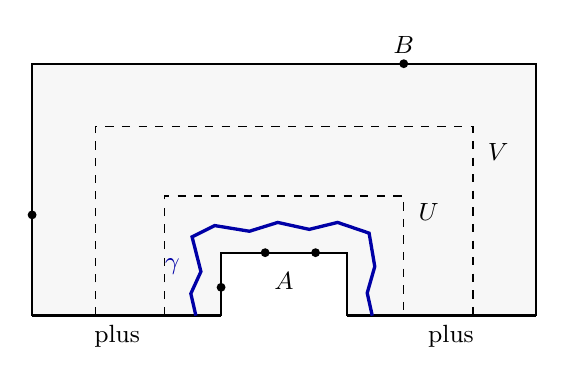
\begin{tikzpicture}[scale=.8, every node/.style={font=\small}]
 \fill[black!3] (-4,0)--(-4,4)--(4,4)--(4,0)--(1,0)--(1,1)
                  --(-1,1)--(-1,0)--cycle;
 \draw[thick] (-4,0)--(-4,4)--(4,4)--(4,0);
 \draw[thick] (-1,0)--(-1,1)--(1,1)--(1,0);
 \draw[very thick] (-4,0)--(-1,0) (1,0)--(4,0);
 \draw[dashed] (-1.9,0)--(-1.9,1.9)--(1.9,1.9)--(1.9,0);
 \draw[dashed] (-3,0)--(-3,3)--(3,3)--(3,0);
 \draw[very thick,blue!65!black]
  (-1.4,0)--(-1.48,.35)--(-1.32,.7)--(-1.46,1.25)
  --(-1.1,1.43)--(-.55,1.34)--(-.1,1.48)--(.4,1.37)
  --(.85,1.48)--(1.35,1.31)--(1.44,.78)--(1.32,.36)--(1.4,0);
 \fill (-1,.45) circle (2pt) (-.3,1) circle (2pt)
       (.5,1) circle (2pt);
 \fill (-4,1.6) circle (2pt) (1.9,4) circle (2pt);
 \node at (0,.55) {$A$};
 \node[above] at (1.9,4) {$B$};
 \node[anchor=west] at (1.98,1.65) {$U$};
 \node[anchor=west] at (3.08,2.6) {$V$};
 \node[blue!65!black,anchor=east] at (-1.5,.78) {$\gamma$};
 \node[below] at (-2.65,0) {plus};
 \node[below] at (2.65,0) {plus};
\end{tikzpicture}
\caption{The dual shell in the free-side argument. The insertion sets
$A,B$ lie at the terminal caps, and $U,V$ are buffered cuts. An open
screen $\gamma$ joins the two plus sides between $A$ and $U$.
Revealing it from the $U$ side leaves the ordinary FK law on its
insertion side, with the screen wired plus. The drawing is schematic.}
\label{fig:boundary-screen}
\end{figure}

We claim the uniform bounds
\begin{equation}
 \|F_A\|_\infty\le C\langle s_A\rangle_*,
 \qquad
 \|F_B\|_\infty\le C\langle s_B\rangle_*.
 \label{eq:buffered-insertion-bound}
\end{equation}
The constant must be independent of the number of insertions.
This is why an absolute correlation estimate alone would not prove
the desired projective bound.

Here is an FK proof of \eqref{eq:buffered-insertion-bound}. For an
insertion set $A$, let $\mathcal E_A$ be the event that every open
cluster not meeting a pinned vertex meets $A$ an even number of times.
With all pins plus, Edwards--Sokal gives
$\langle s_A\rangle=\phi(\mathcal E_A)$. The event
$\mathcal E_A$ is increasing: merging two admissible unpinned clusters
preserves even parity, and joining a cluster to the pins removes its
parity constraint. For arbitrary signs on the cut, the FK edge law
is the law with all pins wired, conditioned on there being no actual
open path between differently signed pins. This follows by counting
the free spin choices of clusters. The conditioning event is
decreasing; paths in this statement use edges of the graph, not the
external wiring. If $m_A^{\mathrm{cut},+}$ denotes the insertion
expectation with the cut pinned plus, Edwards--Sokal and FKG give
\begin{equation}
   |\langle s_A\mid U=u\rangle_*|
       \le\phi_{\mathrm{plus\ cut}}(\mathcal E_A)
       =m_A^{\mathrm{cut},+}.
 \label{eq:insertion-plus-cut}
\end{equation}

To compare this quantity with the uncut expectation, require an open
transverse crossing in a proportional buffer between $A$ and the cut,
joining the two plus-pinned rays. Pure FK-Ising RSW gives this event
probability at least $c>0$, uniformly in exterior boundary conditions
\cite{CDH}. Reveal an outermost such crossing $\gamma$ from the cut
side. This screen separates the insertions from the cut and is connected
to the plus pins. Conditional on the reveal, its insertion side has
the ordinary FK law with $\gamma$ wired plus.

The nearer wired screen increases the parity-event probability, even
for an arbitrarily large insertion set. Indeed restrict the farther
plus-cut law to the region between the terminal and $\gamma$.
Its induced partition is dominated by full wiring on $\gamma$.
The farther-cut parity event implies the near-region parity event
where all clusters touching $\gamma$ are exempt. Since this latter
event is increasing, its probability with $\gamma$ wired is at least
$m_A^{\mathrm{cut},+}$. In the uncut law the revealed screen is actually
connected to the plus rays, so the near-region parity event implies
the full parity event. Hence
\[
 \langle s_A\rangle_*
     \ge c\,m_A^{\mathrm{cut},+}.
\]
Together with \eqref{eq:insertion-plus-cut}, this proves
\eqref{eq:buffered-insertion-bound}; the other cap is identical.
Fixed-shape buffers give the same argument in corner sectors.

The joint law of $U,V$ is a positive left factor, the intervening
pinned-ray kernel, and a positive right factor. If that kernel has
projective diameter $a$, its normalized conditional rows differ by
relative factors in $[e^{-a},e^a]$. Averaging a row over the first
marginal gives
\begin{equation}
 e^{-a}\le
 \frac{\mathbb P(U=u,V=v)}{\mathbb P(U=u)\mathbb P(V=v)}
 \le e^a.
 \label{eq:cut-relative-density}
\end{equation}
For the straight shell we have $a\le Cd^{-2}$. The spin Markov
property makes the two insertion regions conditionally independent
given $U,V$. Thus \eqref{eq:buffered-insertion-bound} and
\eqref{eq:cut-relative-density} imply
\begin{align*}
 \big|\langle s_A s_B\rangle_*
            -\langle s_A\rangle_*\langle s_B\rangle_*\big|
 &\le (e^a-1)\,\mathbb E|F_A(U)|\,\mathbb E|F_B(V)|\\
 &\le C d^{-2}\langle s_A\rangle_*\langle s_B\rangle_*.
\end{align*}
For sufficiently large fixed $d$ this is relative factorization with
error less than $1/2$, uniformly over both insertion sets. Substitution
in \eqref{eq:free-boundary-duality} proves the asserted bound for
$\overline T$. In a corner, choose the fixed ratio large enough that
the pinned-ray diameter is small; the identical argument gives the
finite bound for the free-ray quotient kernel.

\paragraph{A change of boundary condition.}
It remains to bound a shell with one plus ray and one free ray.
Enlarge the terminal groups along both rays as in the pinned case.
The added spins on the free ray may first be conditioned upon and
then summed out; summation preserves the resulting projective bound.
Supermodularity again reduces the problem to the extreme terminal
assignments. The domain-wall expansion used in
\eqref{eq:free-boundary-duality} now has one dual plus ray.
Indeed, after the terminal enlargement the remaining free primal
segment is the same in all four extreme assignments, so its dual
plus ray and its endpoints are unchanged. Reversing a terminal
creates one prescribed wall end where that terminal meets the pinned
primal ray; at its other endpoint walls may end on the free primal
segment without a parity constraint. Thus the terminal assignments
$++,+-,-+,--$ give source sets
$\varnothing,\{y\},\{x\},\{x,y\}$, respectively, in one fixed dual
model. Cancelling the separate terminal factors expresses their
cross ratio as
\begin{equation}
 \frac{\langle s_xs_y\rangle_*}
      {\langle s_x\rangle_*\langle s_y\rangle_*}.
 \label{eq:mixed-boundary-ratio}
\end{equation}
There are just two insertions, at the switches on the pinned primal
ray. Their dual neighborhoods are locally straight and free, and
are a positive distance from each other and from the dual plus ray.
All these distances are fixed proportions of the shell geometry.

Choose disjoint half-box neighborhoods $D_x,D_y$ of these sites,
each with several separated concentric half-boxes inside it. Let
$q_x$ be the probability, in $D_x$ with its artificial outer cut wired,
that $x$ has an actual open arm to a fixed inner radius $\rho_x$.
The true straight boundary remains free. Define $q_y$ likewise.
In the Edwards--Sokal expression for $\langle s_xs_y\rangle_*$,
either the two sites are in the same cluster or both are joined to
the plus pins. Either possibility requires the two local arms.
Conditional on all edges outside one neighborhood, full wiring of
its artificial cut dominates the induced partition. Applying this
bound successively in the two disjoint neighborhoods gives
\begin{equation}
             \langle s_xs_y\rangle_*\le q_xq_y.
 \label{eq:mixed-two-arm-upper}
\end{equation}

We next justify the reverse one-point comparison
\begin{equation}
       \langle s_x\rangle_*\ge c q_x,
       \qquad \langle s_y\rangle_*\ge c q_y.
 \label{eq:mixed-one-arm-lower}
\end{equation}
Choose the nested radii, for example, as
$\rho/2,3\rho/4,\rho,2\rho,3\rho,6\rho$, with the artificial cut
at the last radius. In the uncut model require a transverse open
screen in the half-annular band between $2\rho$ and $3\rho$, and
connect it to the actual plus boundary on its outer side. A fixed
chain of overlapping corridors, together with a radial crossing that
must meet the transverse crossing, realizes these requirements.
RSW and FKG give a positive lower bound independent of the mesh.
Reveal the outermost screen from outside, including its connection
to the plus pins; the reveal does not inspect edges on the inner side.

Inside the screen, full wiring of this nearer cut dominates every
partition induced from the farther wired cut at radius $6\rho$.
Hence the conditional probability of an arm to radius $\rho$ is
at least $q_x$. Extending this arm to the screen costs only another
constant. Indeed require a transverse primal crossing in the smaller
half-annular band between $\rho/2$ and $3\rho/4$ and extend it through
overlapping deterministic corridors to beyond radius $3\rho$.
Every arm from the site to radius $\rho$ meets the transverse crossing.
All these requirements are increasing, so FKG and RSW give their
joint occurrence with the arm at a fixed positive fraction of its
probability. An irregular revealed screen causes no loss: it stays
between the prescribed radii, and a corridor crossing continuing
beyond those radii must first reach it. Equivalently, use free
boundary conditions in a deterministic larger half-box for the
crossing lower bound; the law with the nearer screen wired dominates
on the shared edges, since all exterior attachments meet that wired
cut. This proves \eqref{eq:mixed-one-arm-lower}.

Equations \eqref{eq:mixed-two-arm-upper} and
\eqref{eq:mixed-one-arm-lower} bound \eqref{eq:mixed-boundary-ratio}
above by $c^{-2}$. Griffiths' inequality bounds it below by $1$.
The extreme-comparison reduction therefore gives a finite projective
diameter in the mixed case.

Every use of a continuum limit above involves a fixed finite list of
ratios and straight marked boundary pieces. The corresponding locally
regular approximations include rounded caps and bounded layer shifts.
If uniformity over these approximations failed, a violating sequence
with the same limiting polygon and straight marked pieces would
contradict that convergence theorem. Taking the finest threshold for
the finite list of shapes proves the stated uniformity.
\end{proof}

\subsection{Conditional expectations and positive weights}

The kernel estimate concerns whole spin vectors, rather than individual
spins. It therefore transfers directly to a function of an entire
inner patch. We record also the logarithmic version needed when that
function is a possibly large perturbation of the energy.

\begin{corollary}
\label{cor:boundary-observables}
Let a spin patch of diameter at most $r$ be separated from prescribed
remote spins $\zeta$ by pure shells of one of the types in
Lemma~\ref{lem:boundary-transfer}, out to distance $R=dr$.
Allow fixed proportional buffers around the patch and the outer cut.
Let $H$ be a bounded real function of the patch spins and of any
independent auxiliary variables in the patch. In the free/free case
assume that the region inside the shell has no pinned spins and that
$H$ is invariant under reversal of all its spin arguments.
There are constants $C<\infty$ and $\eta>0$ such that
\begin{align}
 \mathop{\mathrm{osc}}_\zeta\mathbb E_{\mathrm{pure}}[H\mid\zeta]
       &\le C a(d)\|H\|_\infty,
       \label{eq:boundary-expectation-transfer}\\
 \mathop{\mathrm{osc}}_\zeta
        \log\mathbb E_{\mathrm{pure}}[e^H\mid\zeta]
       &\le C a(d)\|H\|_\infty,
       \label{eq:boundary-log-transfer}
\end{align}
where $a(d)=d^{-2}$ at a straight homogeneous side and
$a(d)=d^{-\eta}$ at a corner or boundary-condition change.
Here $\mathop{\mathrm{osc}} f=\sup f-\inf f$. The bounds hold for
each fixed sufficiently large $d$ and sufficiently fine mesh, with
thresholds chosen simultaneously for any finite collection of ratios.
\end{corollary}

\begin{proof}
The spin Markov property factors the conditional law across the two
caps into the shell kernel and positive factors on its two sides.
If the shell diameter is $a$, the conditional distributions on the
inner cap, for any two remote conditions, have relative densities in
$[e^{-a},e^a]$. Their mixtures with the conditional law of the inner
patch have the same comparison. With free rays, spin reversal shows
that the distribution of the patch modulo global sign depends only
on the outer spin vector modulo sign. Thus the quotient kernel gives
precisely this comparison for even functions, even when the remote
spins were specified with absolute signs. Integrating independent
auxiliary variables preserves all the bounds.

At a straight side, \eqref{eq:straight-boundary-transfer} now yields
\eqref{eq:boundary-expectation-transfer}. It also bounds the
oscillation of the logarithm of the expectation of any positive
function by $Cd^{-2}$. To retain the factor $\|H\|_\infty$ when
$\|H\|_\infty\le1$, apply relative-density comparison to $e^H-1$;
its supremum norm is at most $e\|H\|_\infty$, while all expectations
of $e^H$ are at least $e^{-1}$. When $\|H\|_\infty>1$, the direct
projective bound is already at most $Cd^{-2}\|H\|_\infty$.

At a corner or change point, divide the region into $m$ successive
shells of the fixed ratio in Lemma~\ref{lem:boundary-transfer}, with
$m\ge c\log d-C$. A diameter bound $D<\infty$ gives a common
positive fraction $e^{-D}$ in every pair of normalized rows.
Consequently conditional expectation contracts oscillation by at most
$q=1-e^{-D}<1$ through each shell. Composition gives a bound
$Cq^m\|H\|_\infty$, which is \eqref{eq:boundary-expectation-transfer}
for some $\eta>0$. The quotient by sign is preserved at every free
shell.

For \eqref{eq:boundary-log-transfer} with $\|H\|_\infty\le1$,
apply the same contraction to $e^H$ and then use the lower bound
$e^{-1}$. For $\|H\|_\infty>1$, first pass through one shell.
The resulting positive function $h$ satisfies
$\mathop{\mathrm{osc}}\log h\le D$, independently of the size of
$H$. Multiplying $h$ by a constant, arrange $1\le h\le e^D$.
The remaining shells contract its ordinary oscillation to at most
$q^{m-1}(e^D-1)$ and preserve its lower bound $1$. Its logarithmic
oscillation has the same upper bound. Absorbing the first shell into
the constant gives $Cd^{-\eta}\le Cd^{-\eta}\|H\|_\infty$.
This argument uses no exponential moment assumption on $\|H\|_\infty$.
\end{proof}
